%%%%%%%%%%%%%%%%%%%%%%%%%%%%%%%%%%%%%%%%%%%%%%%%%%%%%%%%%%%%%%%%%%%%%%%%%%%%%
%%%                                UNIPLOT                                %%%
%%%%%%%%%%%%%%%%%%%%%%%%%%%%%%%%%%%%%%%%%%%%%%%%%%%%%%%%%%%%%%%%%%%%%%%%%%%%%
\subsubsection{Uniplot}
\label{sec:uiuniplot}
\UNIPLOT{} is a ABB standard plot format with
\index{Plot!Uniplot}
a special set of plot vectors. It is mainly used within existing
Fortran programs. An example is given in figure \nameref{fig:uniplot}.

\input{diagrams/ui_uniplot_list}
\index{UNIPLOT@\UNIPLOT}
\index{PROCESSGROUP@\PROCESSGROUP!Uniplot}


\begin{boxedminipage}[t]{\linewidth}
\begin{alltt}
\DESCRIPTION "Example UNIPLOT";
  ... STUFF HERE ...
\UIMANAGER
  \UNIPLOT
    mech_plot\{ "Plot Mech" \};
  \FORM
    Form_Uniplot \{"Plot Mech", \HELPKEY "Mech_Plot", \HIDECYCLE\}
      ( ( mech_plot ) );
\END \UIMANAGER;

\OPERATOR
  \PROCESS  plot_mech_proc : BATCH \{"plotproc"\};
  \PROCESSGROUP
    mech_prog \{"Mech"\}(output_stream \{\DISPLAY=\NONE\},
                       mech_plot[mechuni] = plot_mech_proc( input_stream );
                     );
\END \OPERATOR;
  ... STUFF HERE ...
\END.
\end{alltt}
\end{boxedminipage}


%\newpage

\begin{figure}[h]
   \begin{center}
      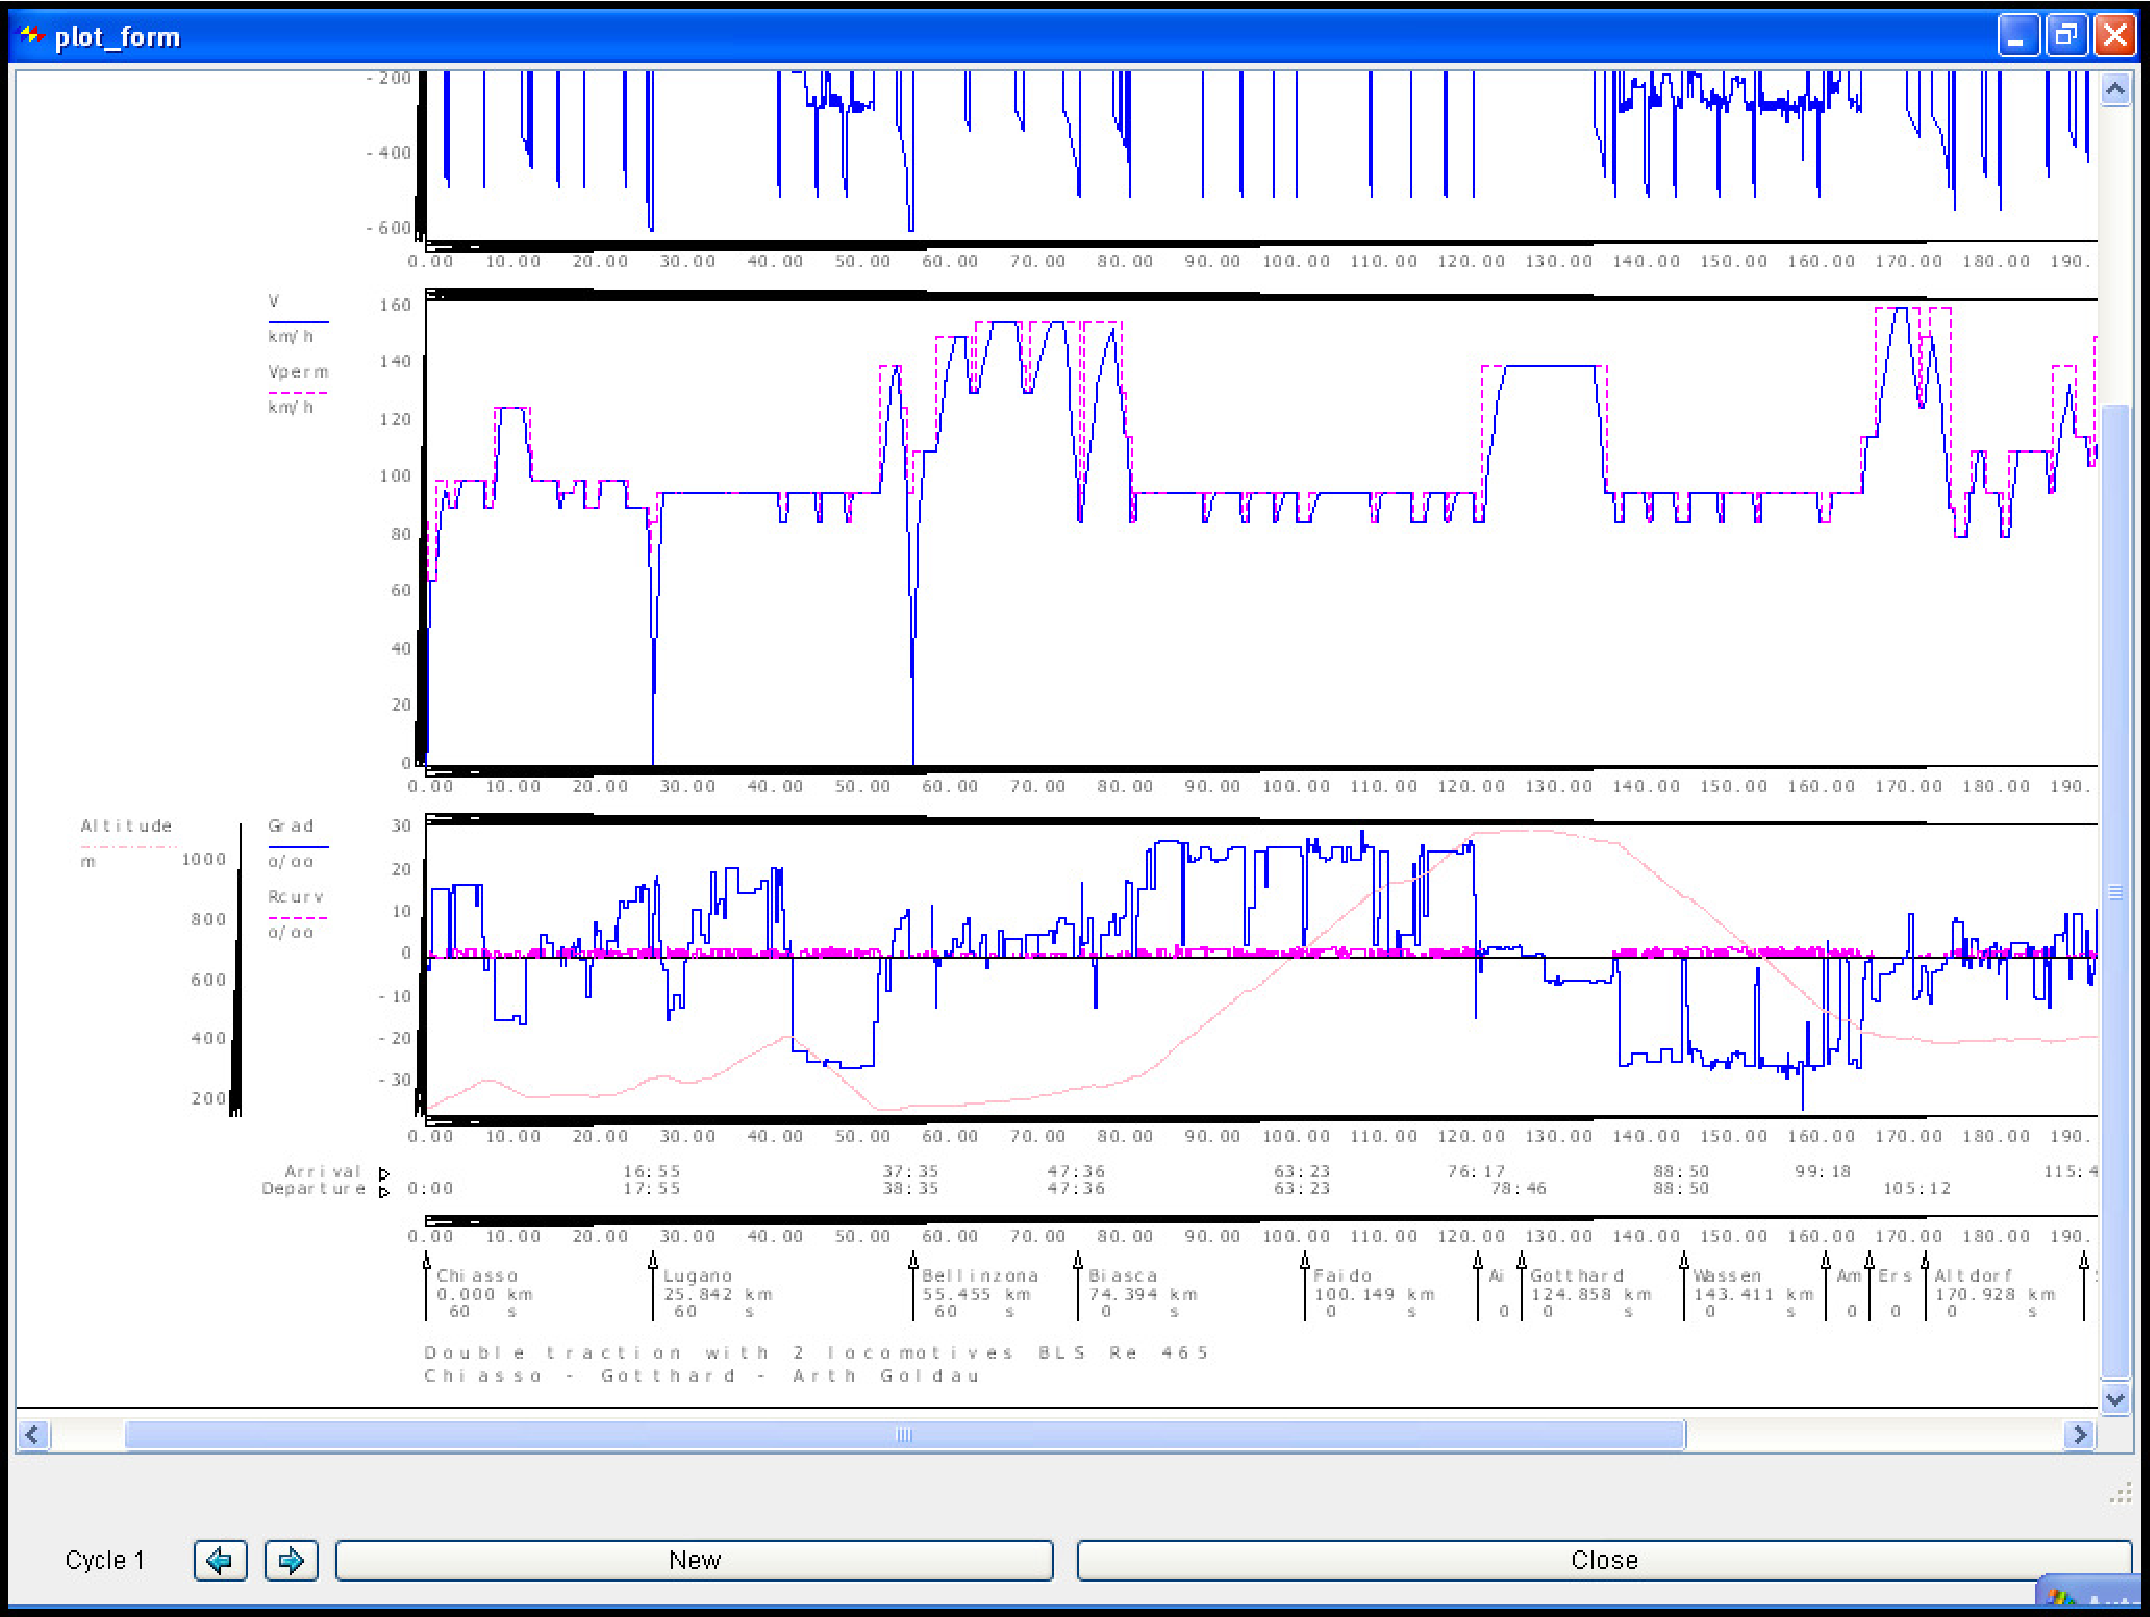
\includegraphics[width=0.8\linewidth]{grab_uniplot}
   \end{center}
\caption{example of a UNIPLOT diagram}
  \label{fig:uniplot}
\end{figure}
